\documentclass{article}

\usepackage{graphicx}
\usepackage{tikz}
\usepackage{tikzsymbols}
\usetikzlibrary{calc,patterns,shapes.geometric}
\pagestyle{empty}
\usepackage[margin=0pt]{geometry}
\geometry{papersize={14in,12in}}

\def\centerarc[#1](#2)(#3:#4:#5){\draw[#1] ($(#2)+({#5*cos(#3)},{#5*sin(#3)})$) arc (#3:#4:#5);}

\begin{document}
	\begin{figure}
		\centering
		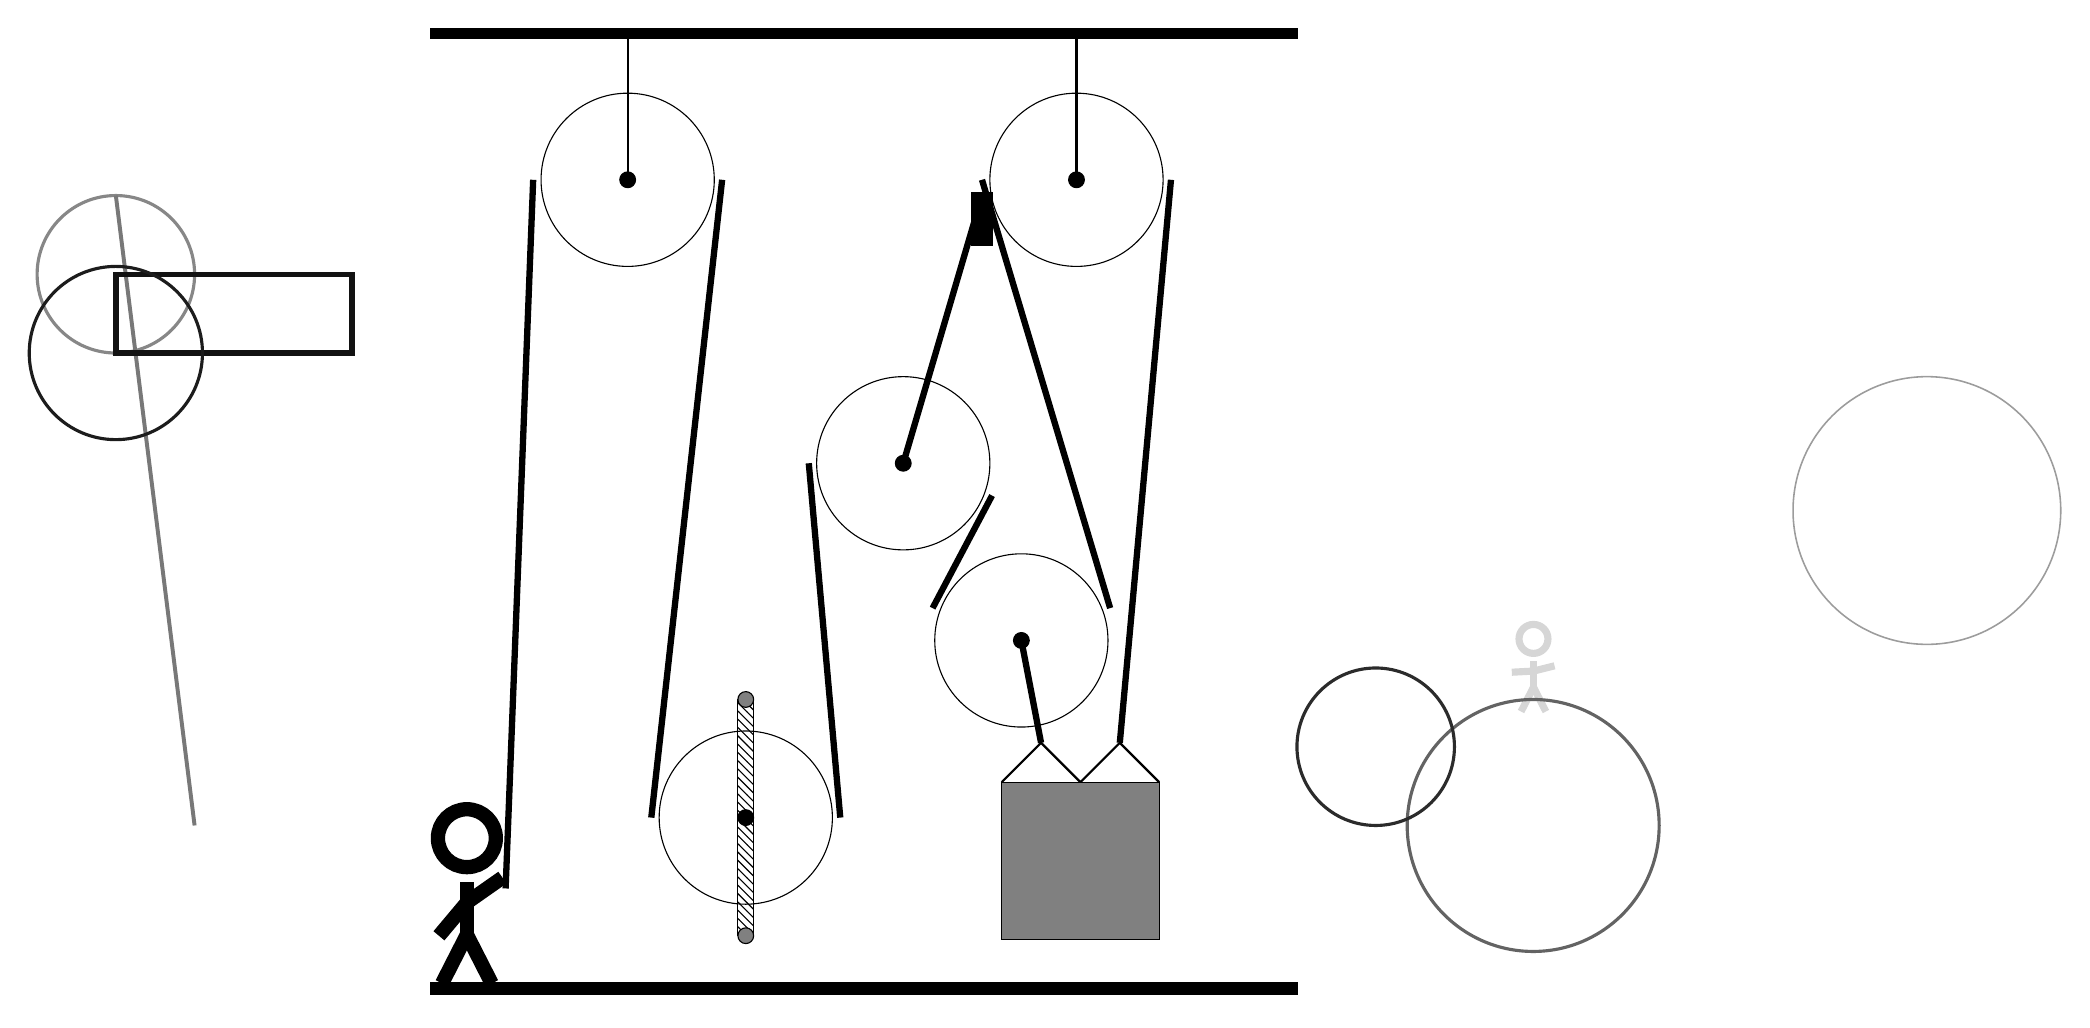
\begin{tikzpicture}
			%%%%% START %%%%%
			
			\draw[fill=black] (-6, 9) rectangle (5, 9.125);
			
			\draw (0, 3.6) circle (1.1);
			\draw[fill=black] (0, 3.6) circle (0.1);
			
			\draw (1.5, 1.35) circle (1.1);
			\draw[fill=black] (1.5, 1.35) circle (0.1);
			
			\node[line width=0.3mm, color=black!16] at (8, 1) {\Strichmaxerl[5][3][14]};
			
			\draw [line width=0.4mm, color=black!47](-10, 6) circle (1.0);
			\draw [line width=0.2mm, color=black!39](13, 3) circle (1.7);
			\draw[line width=0.5mm, color=black!53](-9, -1) -- (-10, 7);
			\draw [line width=0.4mm, color=black!61](8, -1) circle (1.6);
			\draw[line width=0.7mm, color=black!93] (-7, 5) rectangle (-10, 6);
			
			\draw [line width=0.4mm, color=black!83](6, 0) circle (1.0);
			
			\draw [line width=0.4mm, color=black!89](-10, 5) circle (1.1);
			
			\draw (2.2, 7.2) circle (1.1);
			\draw[fill=black] (2.2, 7.2) circle (0.1);
			\draw[thick] (2.2, 7.2) -- (2.2, 9);
			
			\draw (-3.5, 7.2) circle (1.1);
			\draw[fill=black] (-3.5, 7.2) circle (0.1);
			\draw[thick] (-3.5, 7.2) -- (-3.5, 9);
			
			\draw (-2, -0.9) circle (1.1);
			\draw[fill=black] (-2, -0.9) circle (0.1);
			\draw[pattern=north west lines, pattern color=black] (-2.1, 0.6) rectangle (-1.9, -2.4);
			\draw[fill=black!50] (-2, 0.6) circle (0.1);
			\draw[fill=black!50] (-2, -2.4) circle (0.1);
			
			\draw[thick]  (1.25, -0.45) -- (1.75, 0.05) -- (2.25, -0.45) -- (2.75, 0.05) -- (3.25, -0.45);
			\draw[fill=black!50] (1.25, -0.45) rectangle (3.25, -2.45);
			\draw[line width=0.8mm] (-5.05, -1.8) -- (-4.7, 7.2);
			\centerarc[line width=0.8mm](-3.5, 7.2)(0:180:1.2000000000000002);
			\draw[line width=0.8mm] (-2.3, 7.2) -- (-3.2, -0.9);
			\centerarc[line width=0.8mm](-2, -0.9)(180:360:1.2000000000000002);
			\draw[line width=0.8mm] (-0.8, -0.9) -- (-1.2, 3.6);
			\draw[line width=0.8mm] (0, 3.6) -- (1.0, 7.0);
			\draw[line width=0.8mm, fill=black](0.9, 6.4) rectangle (1.1, 7.0);
			\centerarc[line width=0.8mm](0, 3.6)(-20:180:1.2000000000000002);
			\draw[line width=0.8mm] (1.1276, 3.1896) -- (0.3724, 1.7604);
			
			\centerarc[line width=0.8mm](1.5, 1.35)(160:380:1.2000000000000002);
			\draw[line width=0.8mm] (2.6276, 1.7604) -- (1.0, 7.2);
			\draw[line width=0.8mm](1.5, 1.35) -- (1.75, 0.05);
			\centerarc[line width=0.8mm](2.2, 7.2)(0:180:1.2000000000000002);
			\draw[line width=0.8mm] (3.4, 7.2) -- (2.75, 0.05);
			
			\node at (-5.5, -1.9) {\Strichmaxerl[10][50][35]};
			
			\draw[fill=black] (-6, -3) rectangle (5, -3.15);
			
			%%%%% END %%%%%
		\end{tikzpicture}
	\end{figure}	
\end{document}